\documentclass[12pt]{article}

\usepackage{geometry}
 \geometry{
 a4paper,
 total={170mm,257mm},
 left=20mm,
 right=10mm,
 top=10mm,
 bottom=20mm,
 headheight=75pt
 }
% \usepackage[utf8x]{inputenc}
\usepackage{fontspec}
\setmainfont{Open Sans}
\setsansfont{Noto Sans}
\usepackage{graphicx}
\usepackage{forloop}
\usepackage{subcaption}
\usepackage{url}       % `\url`s
\usepackage{floatrow}
\usepackage{hyperref}
\usepackage{cleveref}
\graphicspath{{resources_THEORY/}}

\usepackage{fancyhdr}
\pagestyle{fancy}


\renewcommand{\headrulewidth}{0pt}
% \fancyhead[C]{}
% \fancyfoot[]{}


\newcommand\pic[1]{(\cref{#1})} %Где нужно сослаться на рисунок

\hypersetup{
    colorlinks=true,
    linkcolor=blue,
    urlcolor=cyan,
    }

    \newcommand\ttask[2]{
        \begin{center}
            \LARGE <<Introduction to Mechanical Engineering>> \\ \textbf{Final Exam} \\ \textit{Theory part} \\
            Question: 1 (8 score) \\ Variant: #1
        \end{center}
    #2
    \newpage
    }


    \newcounter{themenumber}

% The preamble ends with the command \begin{document}
\begin{document}
\ttask{1}{\begin{enumerate}
    \item What does it mean? You should explain each part of this notation \pic{fig:resources_THEORY/quiz1_task1.png} (4 score).
    \item Using which 4 basic operations you can design almost any solid part in CAD. Explain your choice with an example (4 score).
\end{enumerate}
\begin{figure}[H]
    \centering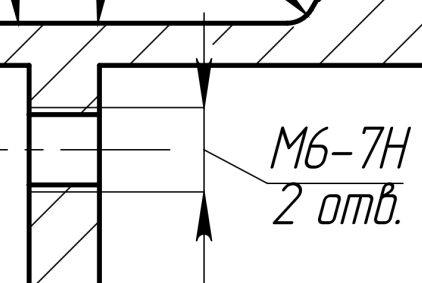
\includegraphics[height=3cm,width=1\textwidth,keepaspectratio]{resources_THEORY/quiz1_task1.png}
    \caption{Variant 1.1}
    \label{fig:resources_THEORY/quiz1_task1.png}
\end{figure}}

\ttask{2}{
\begin{enumerate}
    \item What the difference between lower and higher kinematic pairs and. Provide examples of both types, using kinematic scheme notation (5 score).
    \item Draw a kinematic scheme of the mechanism \pic{fig:resources_THEORY/quiz1_task2.png} (3 score).
\end{enumerate}
\begin{figure}[H]
    \centering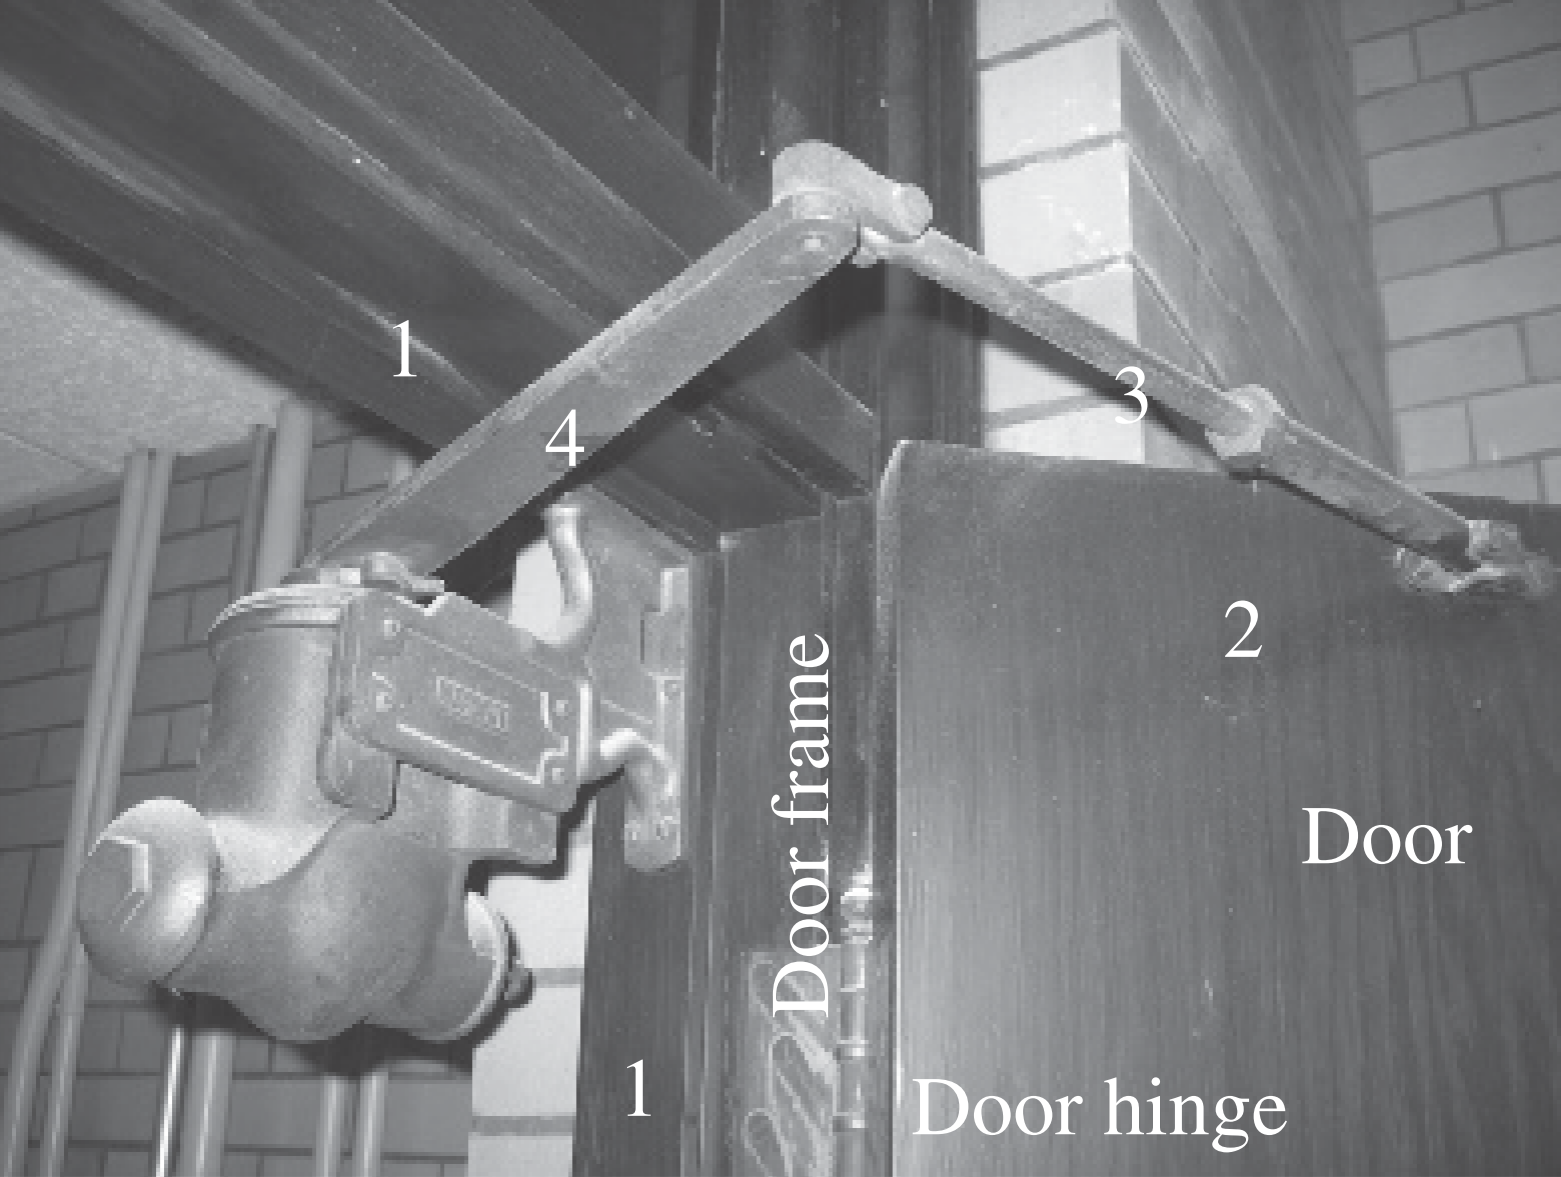
\includegraphics[height=9cm,width=1\textwidth,keepaspectratio]{resources_THEORY/quiz1_task2.png}
    \caption{Variant 2.2}
    \label{fig:resources_THEORY/quiz1_task2.png}
\end{figure}}

\ttask{3}{
\begin{enumerate}
    \item Provide at least 6 types of drives. Prof and cons (8 score).
\end{enumerate}}

\ttask{4}{
\begin{enumerate}
    \item Why do we need bearings? (2 score)
    \item Explain how linear bearings works. (2 score)
    \item How to fix radial bearing on a shaft. At least 2 possible ways. (2 score)
    \item Tolerances for mounting, why do we need them? (2 score)
\end{enumerate}}

\ttask{5}{
\begin{enumerate}
    \item Could you name all highlighted parts from the picture \pic{fig:resources_THEORY/quiz1_task5.png}? (3 score)
    \item What the difference between bolden and direct extruders. (2 score)
    \item Could you write the printing process, starting that you have \textit{ideal} CAD model in <<step>> format. (3 score)  
\end{enumerate}
\begin{figure}[H]
    \centering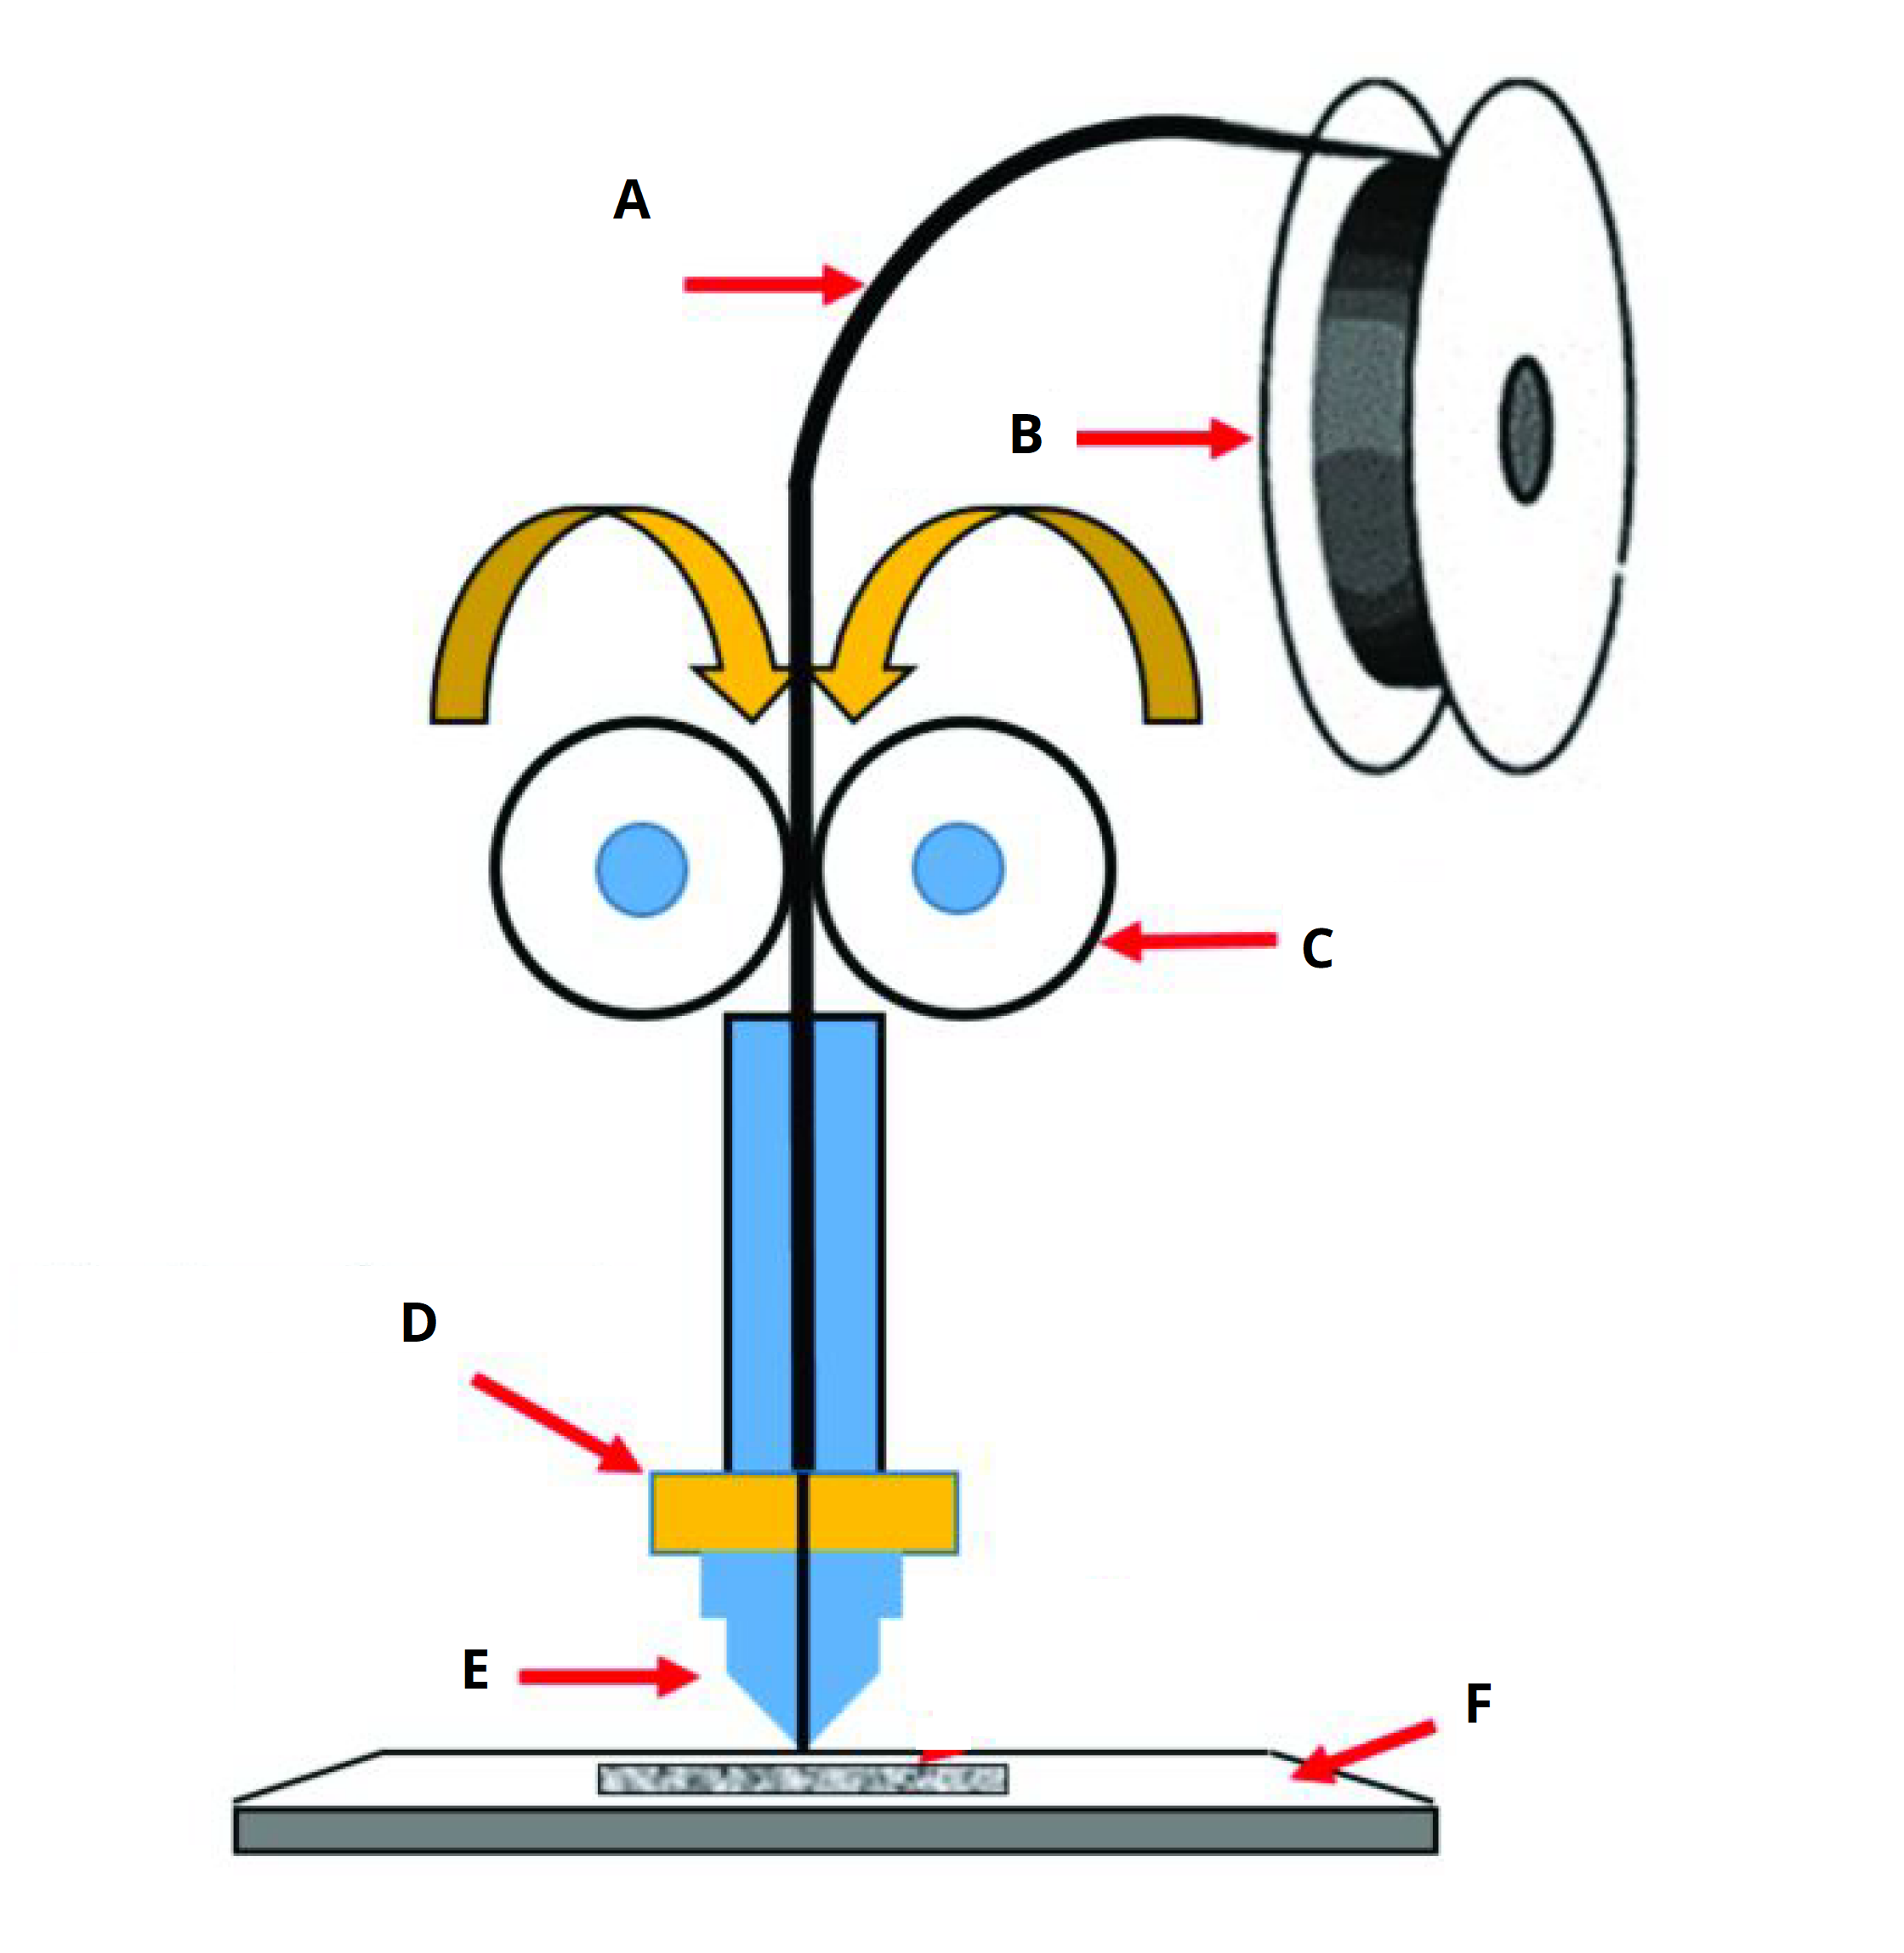
\includegraphics[height=10cm,width=1\textwidth,keepaspectratio]{resources_THEORY/quiz1_task5.png}
    \caption{Variant 5.1}
    \label{fig:resources_THEORY/quiz1_task5.png}
\end{figure}}

\ttask{6}{
\begin{enumerate}
    \item What does stress and strain mean? Stress-strain curve. What the idea besides it? Draw some curve for ductile and brittle material. How can we modify a curve behavior for some particular material? (3 score)
    \item Why do we need alloying elements? Could you provide at least 1 example? (2 score)
    \item Iron-Carbon Phase Diagram \pic{fig:resources_THEORY/quiz1_task6.png}. What can you understand from the diagram? (3 score)
\end{enumerate}
\begin{figure}[H]
    \centering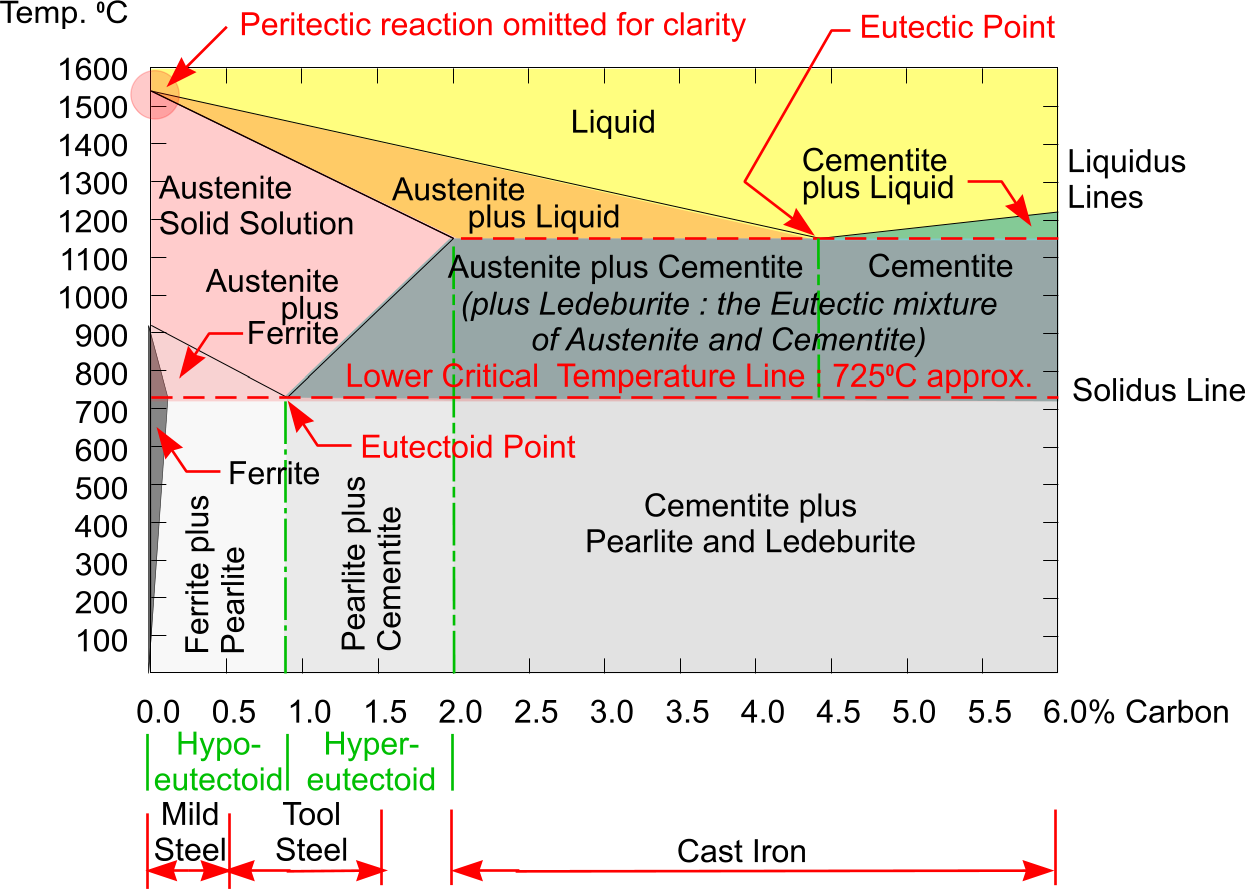
\includegraphics[height=8cm,width=1\textwidth,keepaspectratio]{resources_THEORY/quiz1_task6.png}
    \caption{Variant 6.3}
    \label{fig:resources_THEORY/quiz1_task6.png}
\end{figure}}

\ttask{7}{
    \begin{enumerate}
        \item Could you name each of type connection on the figure \pic{fig:resources_THEORY/final_connections.png}. What the benefits of each of them? (5 score)
        \item How to connect two shafts together? Why do we need it? (3 score)
    \end{enumerate}

    \begin{figure}[H]
        \begin{subfigure}{0.99\textwidth}
            \centering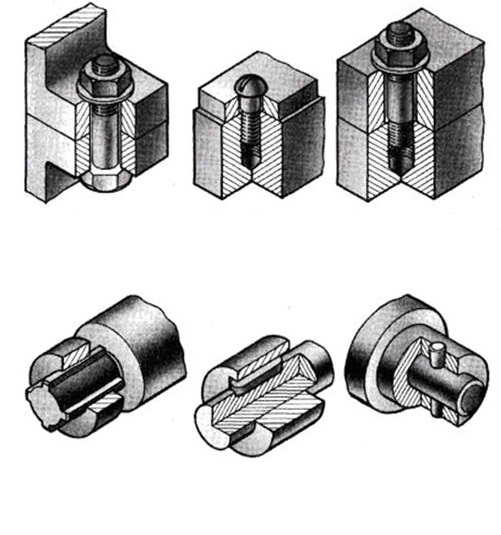
\includegraphics[height=8cm,width=1\textwidth,keepaspectratio]{detach.jpg}
        \end{subfigure}

        \begin{subfigure}{0.99\textwidth}
            \centering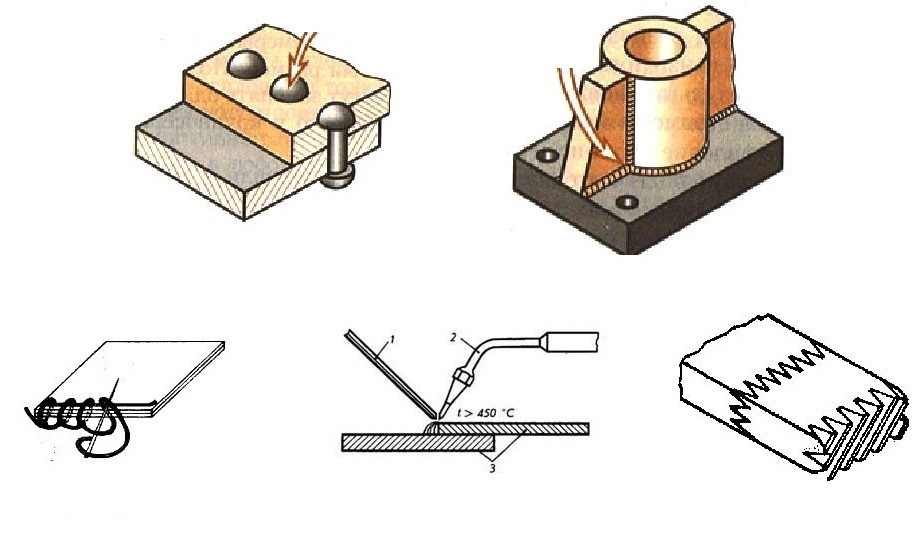
\includegraphics[height=8cm,width=1\textwidth,keepaspectratio]{fixed.jpg}
        \end{subfigure}

    \caption{Variant 7.1}
    \label{fig:resources_THEORY/final_connections.png}
\end{figure}
}

\ttask{8}{
    \begin{enumerate}
        \item What the difference between shaft, spindle and axle? Do we really need different words for them? (2 score)
        \item Screw types. Multiple-Start threads, prof and cons. (1 score)
        \item Screw drive types (шлицы). Prof and cons. (2 score)
        \item Type of drills. Type of holes. How to distinguish them on a blueprints? (1 score)
        \item What the conceptual difference between welding and soldering? Provide the example, where it can be used and why. (2 score)
    \end{enumerate}
}

\forloop{themenumber}{1}{\value{themenumber} < 13}{        \begin{center}
    \LARGE <<Introduction to Mechanical Engineering>> \\ \textbf{Final Exam} \\ \textit{Theory part} \\
    Question: 2 (7 score) \\ Variant: \arabic{themenumber}
\end{center}
\begin{figure}[H]
    \centering\includegraphics[height=10cm,width=1\textwidth,keepaspectratio]{resources_THEORY/MAN1/\arabic{themenumber}.png}
\end{figure}
\newpage
}

\end{document}